\documentclass[11pt]{article}

\newcommand{\cnum}{CM146}
\newcommand{\ced}{Winter 2019}
\newcommand{\ctitle}[3]{\title{\vspace{-0.5in}\cnum, \ced\\Problem Set #1: #2\\Due #3}}
\usepackage{enumitem}
\newcommand{\solution}[1]{{{\color{blue}{\bf Solution:} {#1}}}}
\usepackage[usenames,dvipsnames,svgnames,table,hyperref]{xcolor}
\usepackage{graphicx}
\usepackage[tbtags]{amsmath}


\renewcommand*{\theenumi}{\alph{enumi}}
\renewcommand*\labelenumi{(\theenumi)}
\renewcommand*{\theenumii}{\roman{enumii}}
\renewcommand*\labelenumii{\theenumii.}


\begin{document}
\ctitle{1}{Decision Trees}{Jan 28, 2019}
\author{Tian Ye}
\maketitle

\newpage

\section{Maximum Likelihood Estimation}
\begin{enumerate}
\item 

\solution{
The likelihood estimation is given by the following:
\begin{align}
L(\theta) &= \prod_{i=1}^{n} P_{\theta}(X_{i}) \\
	     &= \prod_{i=1}^{n} \theta^{X_{i}}(1-\theta)^{1-X_{i}} \\
	     &= \theta^{x_{1}}(1-\theta)^{x_{0}}
\end{align}
Where $x_{1}$ counts the number of cases which $X_{i} = 1$ and  $x_{0}$ counts the number of cases which $X_{i} = 0$. \\
The order of the individual random variables $X_{i}$ do not matter as they are independent from one another.
}

\vspace{1cm}

\item
\solution{
Taking the log likelihood of the previous expression:
\begin{align}
\ell(\theta) &= \log(\theta^{x_{1}}(1-\theta)^{x_{0}}) \\
                  &= x_{1}\log(\theta) + x_{0}\log(1-\theta)
\end{align}

Taking the first and second derivatives of $\ell(\theta)$ with respect to $\theta$:
\begin{align}
\ell^{\prime}(\theta) &= \frac{x_{1}}{\theta} - \frac{x_{0}}{1-\theta}\\
\ell^{\prime\prime}(\theta) &= -\frac{x_{1}}{\theta^2} - \frac{x_{0}}{(1-\theta)^2}\\
\end{align}

Since $\ell^{\prime\prime}(\theta) < 0$, the function is always concave down. \\
We can therefore set $\ell^{\prime}(\theta) = 0$ to solve for the MLE:
\begin{align}
\theta_{MLE} = \frac{x_1}{x_{1}+x_0}
\end{align}
}
\newpage


\item
\solution{
\begin{figure}[!htbp]
    \centering
    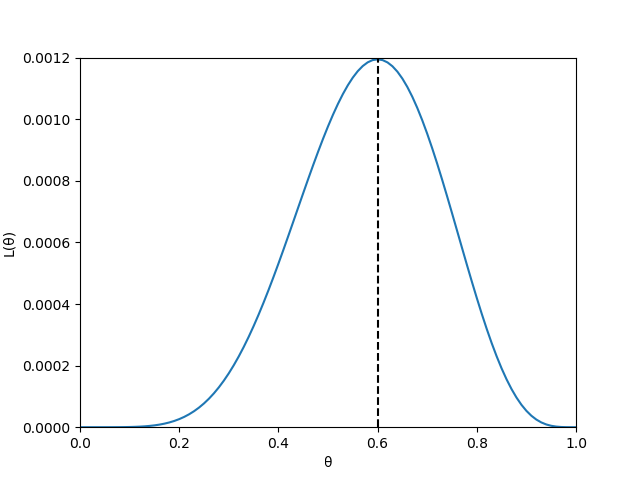
\includegraphics[width=3in]{1c.png}
    \caption{The figure above does agree with Equation 9 given in the previous section; we can see this as the maximum is at $\theta = 0.6$, which corresponds with $\frac{6}{4 + 6}$.}
\end{figure}
}

\item
\solution{
\begin{figure}[!htbp]
    \centering
    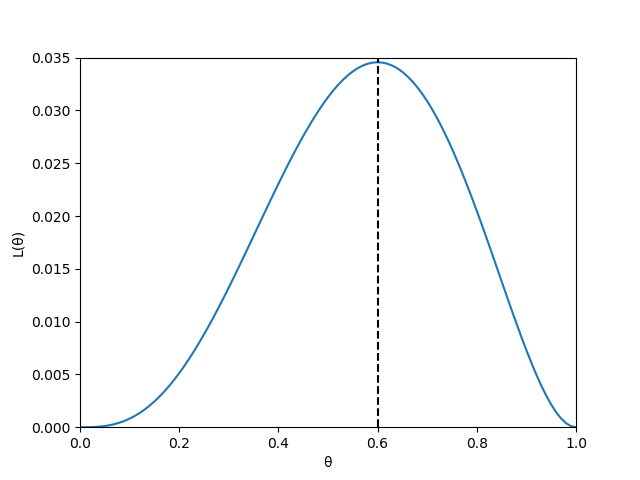
\includegraphics[width=3in]{1di.png}
    \caption{By decreasing the number of data points while maintaining the ratio of 1s to 0s, the likelihood plot keeps the same MLE while having a wider spread but higher likelihood.}
\end{figure}
\newpage

\begin{figure}[!htbp]
    \centering
    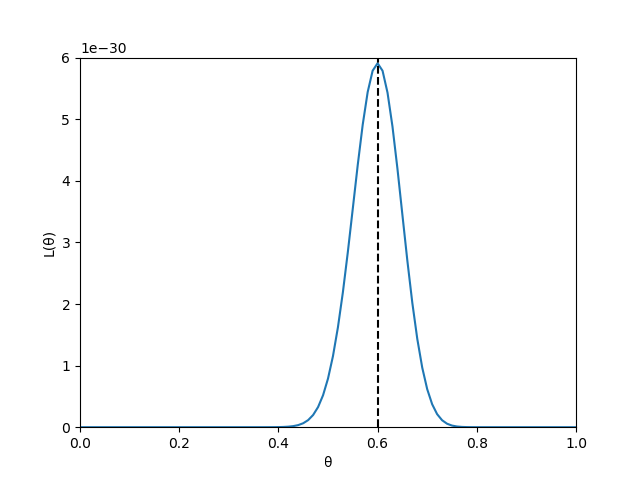
\includegraphics[width=3in]{1dii.png}
    \caption{By increasing the number of data points while maintaining the ratio of 1s to 0s, the likelihood plot keeps the same MLE while having a narrower spread but a lower likelihood.}
\end{figure}

\begin{figure}[!htbp]
    \centering
    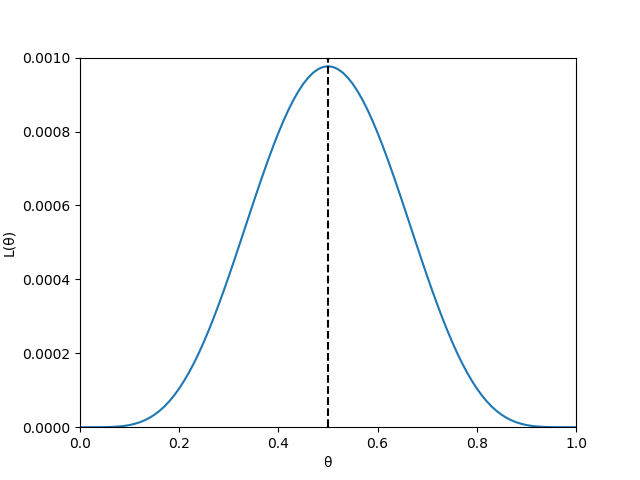
\includegraphics[width=3in]{1diii.png}
    \caption{By maintaining the same number of data points while changing the ratio of 1s to 0s, the likelihood plot shifts the MLE while maintaining the spread and likelihood.}
\end{figure}
}
\end{enumerate}
\newpage

\section{Splitting Heuristic for Decision Trees}
\begin{enumerate}
\item
\solution{The best 1-leaf decision tree makes an error $\frac{1}{8}$ of the time.  The decision tree is as follows: $Y = 0$ if and only if $X_1 = X_2 = X_3 = 0$. \\
This leaves us with $2^{n-3}$ remaining binary vectors; hence the error is $\frac{2^{n-3}}{2^n} = \frac{1}{8}$.
}
\vspace{1cm}

\item
\solution{There does not exist a split that reduces the number of mistakes. If we split on $X_1$, $X_2$, or $X_3$, it will create a tree in which one leaf only contains 1s and the other leaf contains 1s with a proportion of $\frac{3}{4}$. Splitting on a value of $n \geq 4$ will create two leaves where the proportion of 1s is $\frac{7}{8}$. In both cases the tree will always predict 1, leaving an error rate of $\frac{1}{8}$.
}
\vspace{1cm}

\item
\solution{$\frac{1}{8}\log(8) + \frac{7}{8}\log(\frac{8}{5})$ = 0.543
}
\vspace{1cm}

\item
\solution{By splitting on $X_1$, $X_2$, or $X_3$, we can reduce the entropy on the output $Y$. The new entropy following the split is as follows: \\
$\frac{1}{2}[\frac{1}{4}\log(4)+\frac{3}{4}\log(\frac{4}{3})]= 0.406$ \\
This reduces the entropy on $Y$ by 0.137.
}
\newpage
\end{enumerate}

\section{Entropy and Information}
\begin{enumerate}
\item
\solution{We know that the entropy must fall within the range of $0 \leq H(S) \leq 1$ using the following:
\begin{align}
B(q) &= -q\log(q) - (1-q)\log(1-q)
\end{align}
For a set containing $p$ positive examples and $n$ negative examples, $H(S) = B(\frac{p}{n+p})$. We will show that $0 \leq H(S)$ by setting $p=0$ and $n$ to some value greater than 0:
\begin{align}
B(\tfrac{0}{n+0}) &= -q\log(q) - (1-q)\log(1-q) \\
B(0) &= 0\log(0) - (1-0)\log(1-0) \\
H(S) &= 0
\end{align}
For any value of $p$ such that $0 \leq p \leq n$, $H(S)$ increases and approaches 1 as $q$ increases towards $\frac{1}{2}$. Once $p = n$, we yield the following: 
\begin{align}
B(\tfrac{n}{2n}) &= -q\log(q) - (1-q)\log(1-q) \\
B(\tfrac{1}{2}) &= -\tfrac{1}{2}\log(\tfrac{1}{2}) - (1-\tfrac{1}{2})\log(1-\tfrac{1}{2}) \\
H(S) &= 1
\end{align}
As $p$ increases past $n$, the value $q$ once again begins to decrease towards 0, and as such, $H(S)$ decreases back towards 0. Hence, $0 \leq H(S) \leq 1$.
}
\vspace{1cm}

\item
\solution{
}
\end{enumerate}
\end{document}